\documentclass[12pt]{article}
\usepackage[utf8]{inputenc}
\usepackage{amsmath, amssymb}
\usepackage{hyperref}
\usepackage{tikz}
\usepackage[left=2.5cm,right=2.5cm,bottom=2.5cm]{geometry}
\usetikzlibrary{arrows, arrows.meta, positioning, bending, quotes}
\hypersetup{
    colorlinks=true}

\title{MATH 5707 (Spring 2026): Homework 5}
\date{}

\begin{document}
\vspace{-0.7in}

\maketitle
\vspace{-0.6in}


\section*{Directions and Introduction}
Submit a pdf of your solutions to the HW 5 assignment on Gradescope by 11:59 pm on March 20.

Problem 3 is marked as a peer review problem. \href{https://docs.google.com/document/d/1jSw9pmMJJFUx_6dTkcUi4k4HJNIrrIIgs9zdWhAycx0/edit?usp=sharing}{This document gives directions and deadlines for the peer review process.}

When working on this assignment, you should focus on showing fluency with the following skills:
\begin{itemize}
    \item Clearly communicate solutions using complete sentences and enough explanation that another 5707 student could follow your work.
   \item Write formal proofs about graph theoretic topics, including making sure your proofs meet the conventions of mathematical writing (see writing guidelines on Canvas).
    \item 
    Demonstrate fluency with the concept of spanning trees.
    \item Demonstrate fluency with the Matrix-Tree Theorem.
    \item Translating between trees and Pr\"ufer codes. 
    \item Using Laplacian matrices to compute spanning tree enumerator functions.
    \item Using deletion-contraction and/or the matrix tree theorem in a proof.
    \item Translate between Eulerian circuits and last-exit arborescences. 
    \item Apply the BEST Theorem to count the number of Eulerian circuits for a given graph.
\end{itemize}


\section*{Problems}

\begin{enumerate}
\item[0.] If you would like any of these problems to be graded for proficiency with the key skills, list the skill and the corresponding problem.  If you want to label the sill by number, use the numbering that is in the syllabus.
  \item Draw the tree with Pr\"ufer Code $(3,9,8,7,3,1,1)$. 
    \item  Use the Laplacian to compute $t(D,x_0; \underline{a})$ with $x_0=4$ for the digraph  given below. 
    \begin{center}
    
    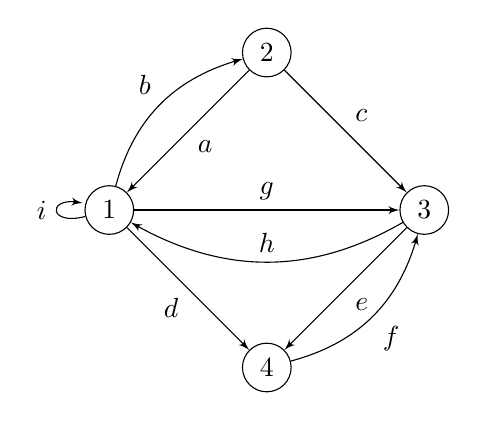
\begin{tikzpicture}

\tikzset{vertex/.style = {shape=circle,draw,minimum size=1.5em}}
\tikzset{every path/.style = {->,> = latex'}}
% vertices
\node[vertex] (a) at  (0,0) {$1$};
\node[vertex] (b) at  (2,2) {$2$};
\node[vertex] (c) at  (4,0) {$3$};
\node[vertex] (d) at  (2,-2) {$4$};
%edges
\path (b) edge["$a$"] (a);
\path (b) edge["$c$"] (c);
\path (a) edge["$d$",swap] (d);
\path (c) edge["$e$"] (d);
\path[bend left] (a) edge["$b$"] (b);
\path[bend left] (c) edge["$h$",swap] (a);

\path (a) edge["$g$"] (c);
\path(a) edge["$i$", loop left] (a);
\path[bend right] (d) edge["$f$",swap] (c);
\end{tikzpicture}
\end{center}

     \item (Bondy-Murty 2.4.5, peer review problem; Each part will be worth 4 points and
graded as a separate problem.)
     \begin{enumerate}
 \item    Choose one of the two following propositions and prove it (if you submit proofs for both propositions, only the first will be graded):
     \begin{itemize}
     \item Let $H$ be a graph in which every two adjacent vertices are joined by $k$ edges and let $G$ be the underlying simple graph of $H$. Show that $t(H)=k^{|V|-1}t(G)$. 
     \item Let $H$ be the graph obtained from a graph $G$ by replacing each edge of $G$ by a path of length $k$. Show that $t(H)=k^{|E|-|V|+1}t(G)$. 
     \end{itemize}
     
     \item Using the two propositions in part (a), prove that $t(K_{2,n})=n2^{n-1}$.  (You can assume both propositions are true even though you only proved one of them.)
     \end{enumerate}

 \item Consider the Eulerian digraph $D$ given below: 
 \begin{center}
     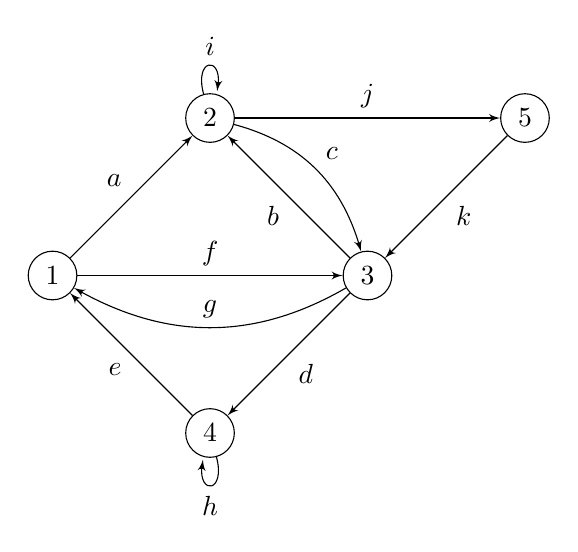
\begin{tikzpicture}

\tikzset{vertex/.style = {shape=circle,draw,minimum size=1.5em}}
\tikzset{every path/.style = {->,> = latex'}}
% vertices
\node[vertex] (a) at  (0,0) {$1$};
\node[vertex] (b) at  (2,2) {$2$};
\node[vertex] (c) at  (4,0) {$3$};
\node[vertex] (d) at  (2,-2) {$4$};
\node[vertex] (e) at  (6,2) {$5$};

%edges
\path (c) edge["$b$"] (b);
\path (d) edge["$e$"] (a);
\path (c) edge["$d$"] (d);
\path (a) edge["$a$"] (b);
\path[bend left] (c) edge["$g$",swap] (a);

\path (a) edge["$f$"] (c);


\path (e) edge["$k$"] (c);


\path[bend left] (b) edge["$c$"] (c);

\path (b) edge["$j$"] (e);





\path(b) edge["$i$", loop above] (b); 

\path(d) edge["$h$", loop below] (d); 
\end{tikzpicture}
\end{center}

\begin{enumerate}
\item Find the last-exit arborescence that corresponds to the Eulerian circuit $$(d,h,e,a,c,g,f,b,i,j,k).$$
\item How many Eulerian Circuits that start and end at vertex $3$ correspond to the following tree? Explicitly list two of them.
 \begin{center}
     \begin{tikzpicture}

\tikzset{vertex/.style = {shape=circle,draw,minimum size=1.5em}}
\tikzset{every path/.style = {->,> = latex'}}
% vertices
\node[vertex] (a) at  (0,0) {$1$};
\node[vertex] (b) at  (2,2) {$2$};
\node[vertex] (c) at  (4,0) {$3$};
\node[vertex] (d) at  (2,-2) {$4$};
\node[vertex] (e) at  (6,2) {$5$};

%edges
\path (b) edge (c);
\path (d) edge (a);
\path (a) edge (c);

\path (e) edge (c);

\end{tikzpicture}

\end{center}
\item Using the B.E.S.T theorem,  find $|\mathcal{E}_D|$.  You may use an online calculator to find the determinant of the necessary Laplacian submatrix and state that result without showing any steps. 
\end{enumerate}



\end{enumerate}

\end{document}